\documentclass[12pt]{scrreprt}  
% Use scrreprt class for reports

%Font Selection
% \usepackage{fontspec}
% \usepackage{times}
% \usepackage{palatino}
% \usepackage{charter}
% \setmainfont{Georgia}
% \setmainfont{Arial}


\usepackage{fontspec}
\setmainfont{Times New Roman}

\usepackage{charter}

\usepackage{graphicx}
\usepackage{array} % For better column control
\usepackage[numbers]{natbib}  % Use natbib for controlling citations
\setlength{\tabcolsep}{12pt}  % Adjusts the padding of the table cells
\renewcommand{\arraystretch}{1.5}  % Adjusts the vertical padding (row height)

% Encoding and languages
\usepackage[utf8]{inputenc}
\usepackage[english]{babel}

% Geometry and page setup
\usepackage[a4paper, margin=1in]{geometry}
\usepackage{float}


\usepackage[utf8]{inputenc}
\usepackage[english]{babel}
\usepackage{hyperref}

% Better handling of URLs and hyperlinks
\usepackage{hyperref}

% Code listings
\usepackage{listings}

% Table management
\usepackage{booktabs}
\usepackage[table,xcdraw]{xcolor}

% Flowchart and diagrams
\usepackage{tikz} 
\usetikzlibrary{shapes, arrows.meta, positioning, backgrounds}

% For easier formatting of captions
\usepackage[justification=centering]{caption}

% For defining acronyms
\usepackage[acronym]{glossaries}

% For rotating tables or figures
\usepackage{rotating}

% SI units handling
\usepackage{siunitx}

% Array handling
\usepackage{array}

% Fancy counters
\usepackage{chngcntr}

% Define styles for different node types
\tikzstyle{startstop} = [rectangle, rounded corners, minimum width=3cm, minimum height=1cm, text centered, draw=black, fill=red!30]
\tikzstyle{process} = [rectangle, minimum width=3.5cm, minimum height=1cm, text centered, draw=black, fill=blue!10]
\tikzstyle{database} = [rectangle, minimum width=3cm, minimum height=1cm, text centered, draw=black, fill=orange!30]
\tikzstyle{auth} = [rectangle, minimum width=3cm, minimum height=1cm, text centered, draw=black, fill=green!30]
\tikzstyle{ui} = [rectangle, minimum width=3.5cm, minimum height=1cm, text centered, draw=black, fill=yellow!30]
\tikzstyle{arrow} = [thick,->,>=stealth]

% For stickman (used in diagrams)
\tikzset{
    stickman/.pic={
        % Head
        \draw[fill=gray] (0,0.6) circle (0.3cm);
        % Body
        \draw[line width=0.5mm] (0,0.3) -- (0,-0.6);
        % Arms
        \draw[line width=0.5mm] (-0.4,0.3) -- (0.4,0.3);
        % Legs
        \draw[line width=0.5mm] (0,-0.6) -- (-0.4,-1.2);
        \draw[line width=0.5mm] (0,-0.6) -- (0.4,-1.2);
    }
}

\hypersetup{
    bookmarks=true,    % show bookmarks bar
    pdftitle={Software Requirement Specification}, % title
    pdfauthor={Jean-Philippe Eisenbarth},         % author
    pdfsubject={TeX and LaTeX},                    % subject of the document
    pdfkeywords={TeX, LaTeX, graphics, images},    % list of keywords
    colorlinks=true,                               % colored links
    linkcolor=blue,                                % color of internal links
    citecolor=black,                               % color of links to bibliography
    filecolor=black,                               % color of file links
    urlcolor=purple,                               % color of external links
    linktoc=page                                   % only page is linked
}


\title{Project proposal format For B.Sc. CSIT/BIT, TU, IOST}
\author{Prakash Neupane}
\date{\today}

\begin{document}
\pagenumbering{roman} % Roman page numbers

% Title page (Design in your own way)

\addcontentsline{toc}{section}{TITLE PAGE}
\thispagestyle{empty} % This will hide page number in title page


% Title page (Design in your own way)

{
	\thispagestyle{empty}
	\centering
	\normalsize
	  
        
\includegraphics[width=1.3in]{Images/PUClogo.png}\\

	{PREMIER UNIVERSITY}\\
	{DEPARTMENT OF COMPUTER SCIENCE AND ENGINEERING}\\
	
	\\[1.5cm]
	{\textit{A Project Report On}\\
	{\bf YOUR project Title Goes Here in UPPER CASE}\\[1.5cm]

     {\bf Course Title:} Software Development\\
     {\bf Course Code:}  CSE 364\\[1.5cm]

        Submitted To:\\
	   Faculty Name \\
          Designation \\
          Department of Computer Science and Engineering\\[1.5cm]
    
	% ~
	
	Submitted By:\\
	{\bf Full Name} (PU Exam Roll No)\\
        {\bf Full Name} (PU Exam Roll No)\\
	{\bf Full name} (PU Exam Roll No)\\[3.5cm]
	% ~
	
	September, 2024
	
}

}

%%% Local Variables:
%%% mode: plain-tex
%%% TeX-master: t
%%% End: % Ensure this file exists and is correctly formatted

% Table of contents
\newpage
{
  \setlength{\parskip}{0em}
  \renewcommand\contentsname{TABLE OF CONTENTS} % This will change heading text
  \tableofcontents \addcontentsline{toc}{section}{TABLE OF CONTENTS}
}

% List of figures - if any
\newpage
\listoffigures 
\addcontentsline{toc}{section}{LIST OF FIGURES}

% List of tables - if any
\newpage
\listoftables 
\addcontentsline{toc}{section}{LIST OF TABLES}
\pagenumbering{arabic}

\newpage
\section{Introduction}
Read some papers to begin and develop your writing style.
This section provides an overview of the project, including its significance and the motivation behind choosing the topic. Explain the broader context and relevance of the project, highlighting its potential impact on a specific field or problem area. Briefly describe what the project aims to achieve and the scope of work involved

Online vehicle rental systems are popular these days~\cite{vehicle}.
In the introduction, provide background information on the topic of your project. Explain the context and relevance of the problem you are addressing. Briefly state the purpose and scope of your project proposal. The introduction should capture the reader's interest and provide a high-level overview of what the proposal will cover~\cite{ref1}
 % Ensure this file exists and is correctly formatted
\section{Problem Statement}
Clearly define the problem or question the project seeks to address.
    
Specify how the solution will be evaluated (e.g., accuracy, speed, precision).


Sample of figure for problem statement:

\url{https://www.pi.exchange/hs-fs/hubfs/KH%20Article%20Assets/image-20230707-054308.png?width=500&height=333&name=image-20230707-054308.png} 
\section{Objectives} 
What problem does this project aim to solve?

Specify the goals and intended outcomes.

\newpage
\section{Methodology}
 Proposed machine learning approach (e.g., supervised learning, unsupervised learning, deep learning).
    
Algorithms/models under consideration.

Tools, libraries, and frameworks you plan to use.

\begin{figure}[h]
    \centering
    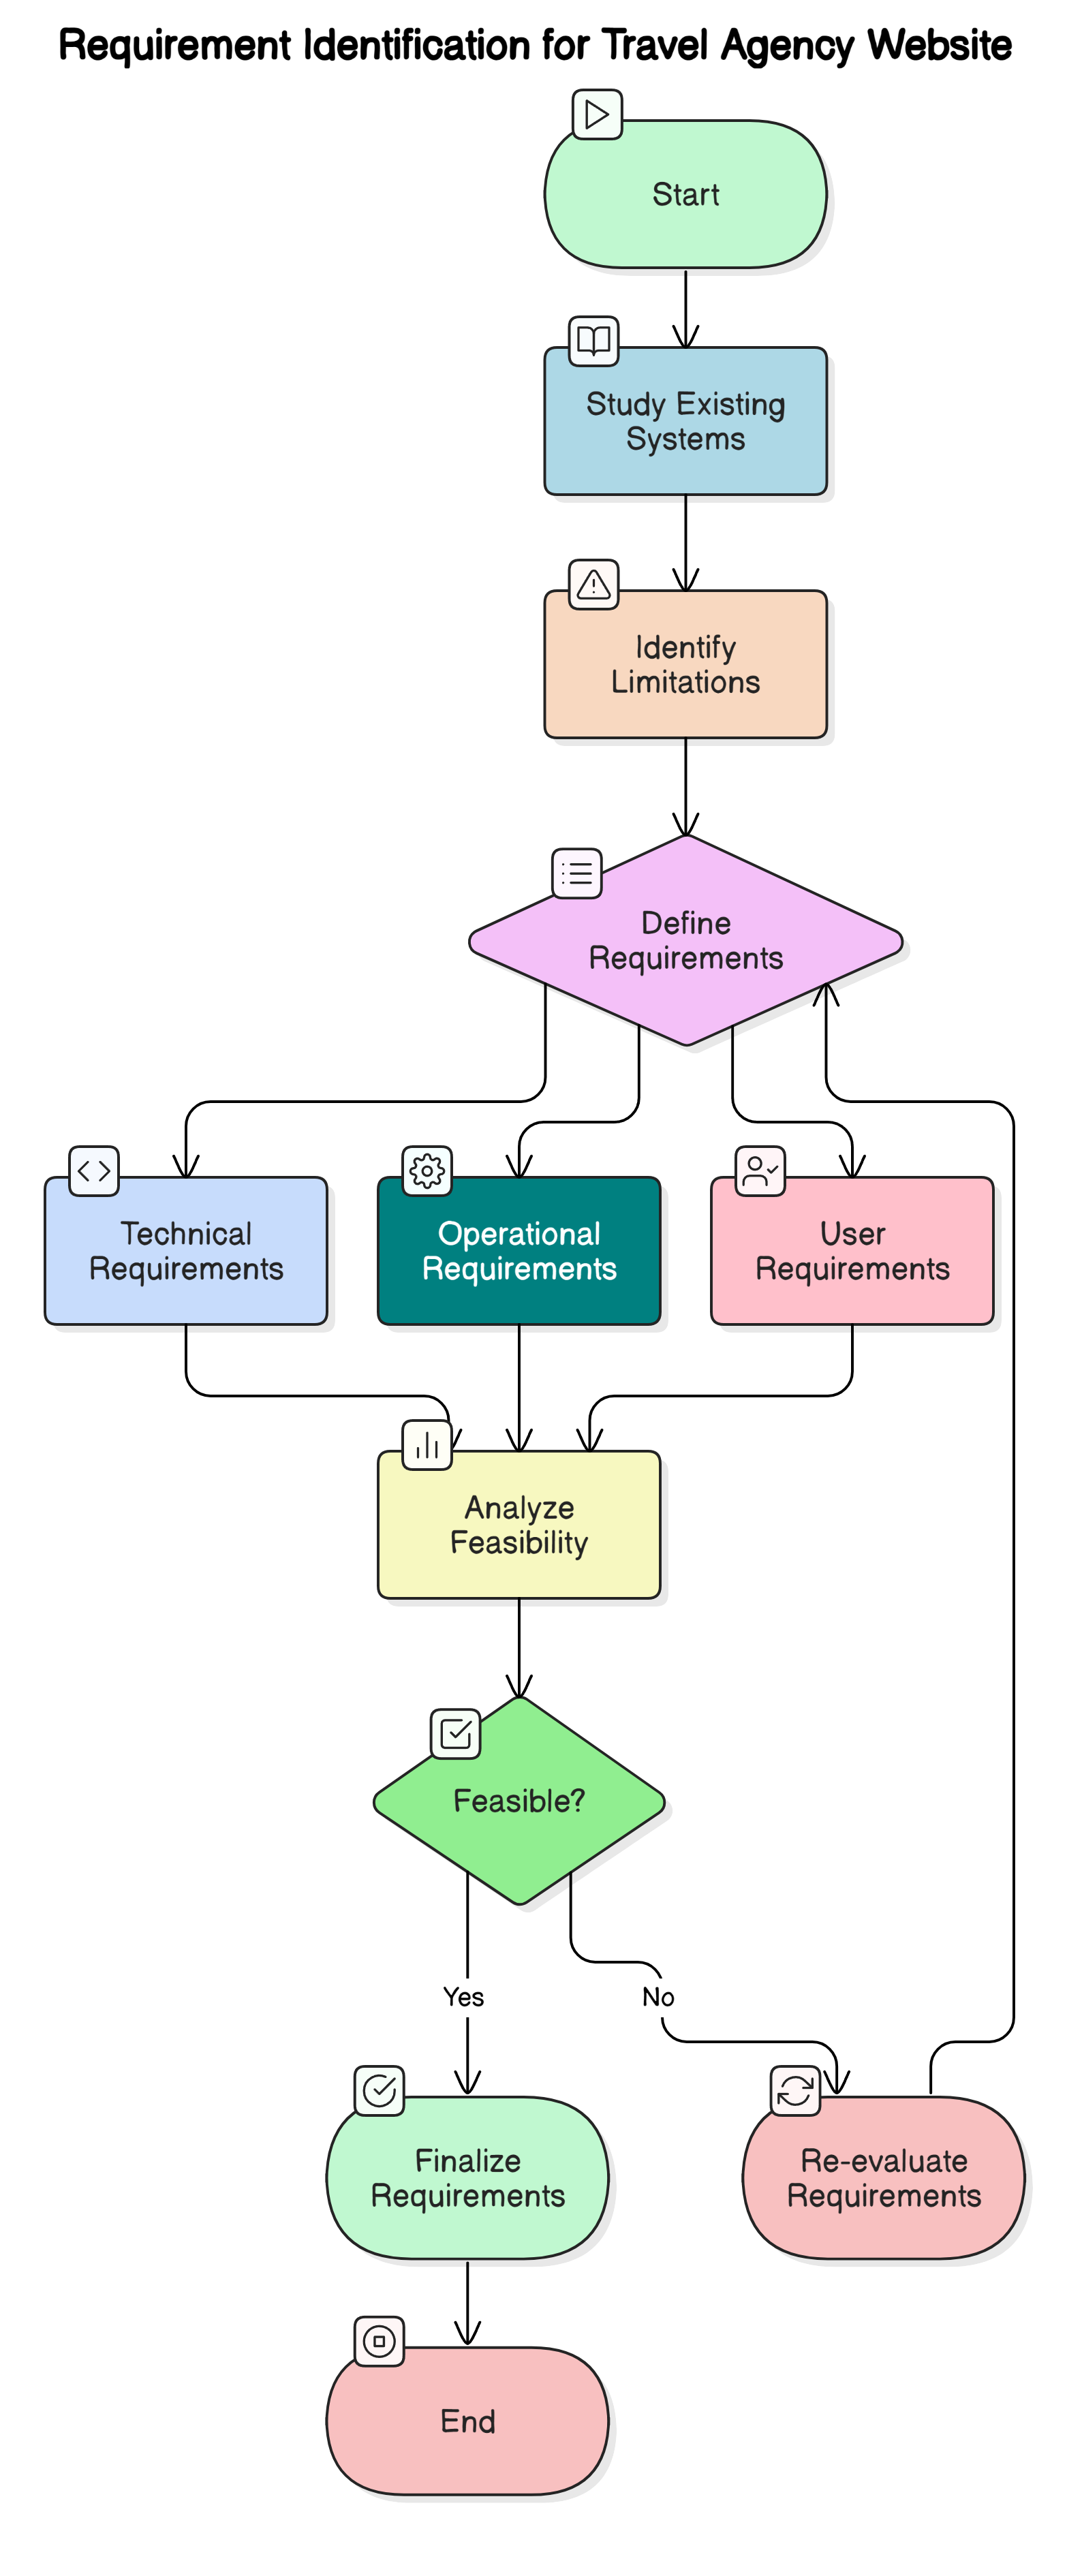
\includegraphics[width=0.5\linewidth]{Images/flow.png}
    \caption{Caption}
    \label{fig:enter-label}
\end{figure}

\begin{table}[h]
    \centering
    \caption{sample Cost-Benefit Analysis of the Proposed Project}
    \begin{tabular}{@{}llcc@{}}
        \toprule
        \textbf{Item} & \textbf{Description} & \textbf{Cost (\$)} & \textbf{Benefit (\$)} \\ \midrule
        Development Costs & Software Development & 15,000 & - \\
        Hardware Costs & Servers and Equipment & 5,000 & - \\
        Training Costs & User Training Sessions & 2,000 & - \\
        Maintenance Costs & Annual Maintenance & 1,000 & - \\
        \midrule
        \textbf{Total Costs} &  & \textbf{23,000} & - \\ \midrule
        Increased Efficiency & Time Savings & - & 30,000 \\
        Improved User Satisfaction & User Feedback & - & 10,000 \\
        Revenue Increase & New Customers & - & 20,000 \\
        \midrule
        \textbf{Total Benefits} &  & - & \textbf{60,000} \\ \midrule
        \textbf{Net Benefit} &  & \textbf{23,000} & \textbf{37,000} \\ 
        \bottomrule
    \end{tabular}
    \label{tab:cost-benefit}
\end{table}

 


\url{https://www.onlinegantt.com/#/gantt} to create a Gantt chart as per our need.
  

\newpage
\input{sec/expected_output}

% References
\phantomsection
\addcontentsline{toc}{section}{REFERENCES}  % Add to Table of Contents

% Citing references
% Add references to bibliography, but do not cite in text
\nocite{ref1, ref2, ref3, ref4, ref5, ref6, ref7}


\bibliographystyle{IEEEtran}  % Choose your bibliography style

\bibliography{biblio}  % Make sure 'biblio' matches the name of your .bib file (without the .bib extension)

\end{document}